
\section{Vers une prise en compte plus générale de l'exposition}

Au cours de ma thèse, plusieurs questions ont pu être adressées et certaines réponses
apportées.  Cependant, le choix a été fait de se limiter principalement sur l'estimation
des sources de PO à travers le modèle PMF. Bien qu'apportant des résultats éclairant sur
la dynamique des PO, plusieurs aspects ont été volontairement écartés de ces études.

Premièrement, l'utilisation de modèle site-récepteur limite nécessairement la couverture
spatiale et temporelle à quelques sites d'études et années de mesures. Or la
généralisation d'une estimation des mesures de PO à tous points spatio-temporel est
souhaitable lorsque l'on s'intéresse à coupler dans une même étude mesures
épidémiologiques et qualité de l'air.

Deuxièmement, la méthode utiliser pour estimer un PO par sources de PM présente un
développement mathématique linéaire. Or, on sait que le PO ne réagit pas de manière
linéaire à la masse des composés chimiques. Si ce modèle présente une première
approximation, il est, par construction, limité et biaisé.  Il existe cependant des
modèles d'inversion non-linéaire qui permettraient la prise en compte des interactions
entre sources et composés chimiques dans l'estimation des sources de PO.

Finalement, jusqu'à présent seuls des prélèvements en air extérieur ont été considérés. Or
nous passons la plus grande partie de notre temps en espace clos intérieur (maison,
appartement, bureau, voiture, etc.).  La représentativité des mesures en air extérieur
comme référence de l'exposition de la population n'est donc peut-être suffisante.

\section{Spatialisation du PO}

\subsection{Estimation du PO à partir des PM}

Dans cette thèse, deux synthèses nationales grande échelle ont été faite : 1) estimation
des contributions des sources de PM à la masse \autocite{weberComparison2019}
(chapitre~\ref{cha:estimation_des_sources_de_PO}) et 2) attribution du PO intrinsèque à
chacune des sources de PM majoritairement présentes \autocite{weberSourceinprep.}
(chapitre~\ref{cha:estimation_des_sources_de_PO}).

Ainsi, et en première approximation, il est possible d'estimer la contribution moyenne
relative mensuelle des différentes sources à la masse totale des PM. Puis, connaissant le
PO intrinsèque (i.e. par microgramme de PM) de chacune de ces sources, une simple
multiplication permet une estimation approximative du PO.  La conséquence est que pour
chaque valeur de concentration de \PMdix{} il est possible d'estimer, au premier ordre,
une valeur de PO associée.

Bien évidemment, cette méthode possède trois limitations fortes : 
\begin{itemize}
    \item Les contributions relatives des sources sont moyennées mensuellement d'après un
        ensemble de 15 sites de mesures, de typologie plutôt urbaine, et donc non
        nécessairement représentative de l'ensemble des situations possibles ;
    \item Le PO intrinsèque de chacune de ces sources présente en réalité une variabilité
        plus ou moins importante, et une fois de plus estimés à partir d'un ensemble de
        site de typologie plutôt urbaine ;
    \item Il n'est pas pris en compte la spécificité du site en question ni la possible
        évolution du PO intrinsèque des sources liés à possible une évolution du profile
        chimique (renouvellement de parc automobile, etc.).
\end{itemize}

Elle présente néanmoins l'avantage de pouvoir estimer pour n'importe quel site possédant
une concentration massique des \PMdix{} une mesure de \POAAv{} et \PODTTv. Il est
également possible d'utiliser ce procédé en post-traitement d'un modèle déterministe de
prévision de concentration de \PMdix.

Aussi, au fur et à mesure que de nouvelle étude se feront, il est tout à fait possible de
raffiner cette technique en ne sélectionnant que des sites de même typologie ou
environnement (rurale, vallée alpine, trafic, etc.) aussi bien pour la partie d'estimation
de la contribution des sources aux \PMdix{} que pour la partie attribution d'un PO
intrinsèque par source.

Afin de tester la faisabilité de cette méthode d'estimation au premier ordre du PO, le
site de Grenoble les Frènes a été choisi car bénéficie d'une série de mesure longue durée
du PO. Cette méthode est aussi rendu disponible grâce au développement du module python
\href{https://gricad-gitlab.univ-grenoble-alpes.fr/pmall/pyopestimator}{pyOPestimator},
disponible sur PyPi\footnote{\url{https://pypi.org/project/pyOPestimator/}} et sur la
forge de l'université de
grenoble\footnote{\url{https://gricad-gitlab.univ-grenoble-alpes.fr/pmall/pyopestimator}}.
Il est également possible d'utiliser directement
\url{http://getopstandop.u-ga.fr/estimate}, permettant d'estimer directement en ligne le
\POAAv{} et \PODTTv{} de n'importe quelle série de mesure concentration de \PMdix.

Les \POAAv{} et \PODTTv{} mesurés et estimés par cette méthode sont présentés
figure~\ref{fig:OPGRE-fr-estimated}.  Les cycles saisonnier sont bien retrouvés et les
amplitudes respectées. Cependant et comme attendu, certains évènements peu fréquent sont
mal estimés. Au final, une corrélation (Pearson) respective de 0.75 et 0.79 pour le
\POAAv{} et \PODTTv{} est obtenu en prenant en compte les 769 échantillons où les PO ont
été mesurés (voir figure~\ref{fig:OPGRE-fr-estimated_scatter}).  Considérant les grandes
approximations faites par cette méthode, ce résultat présente des performance étonnante !

\begin{figure}[ht]
    \centering
    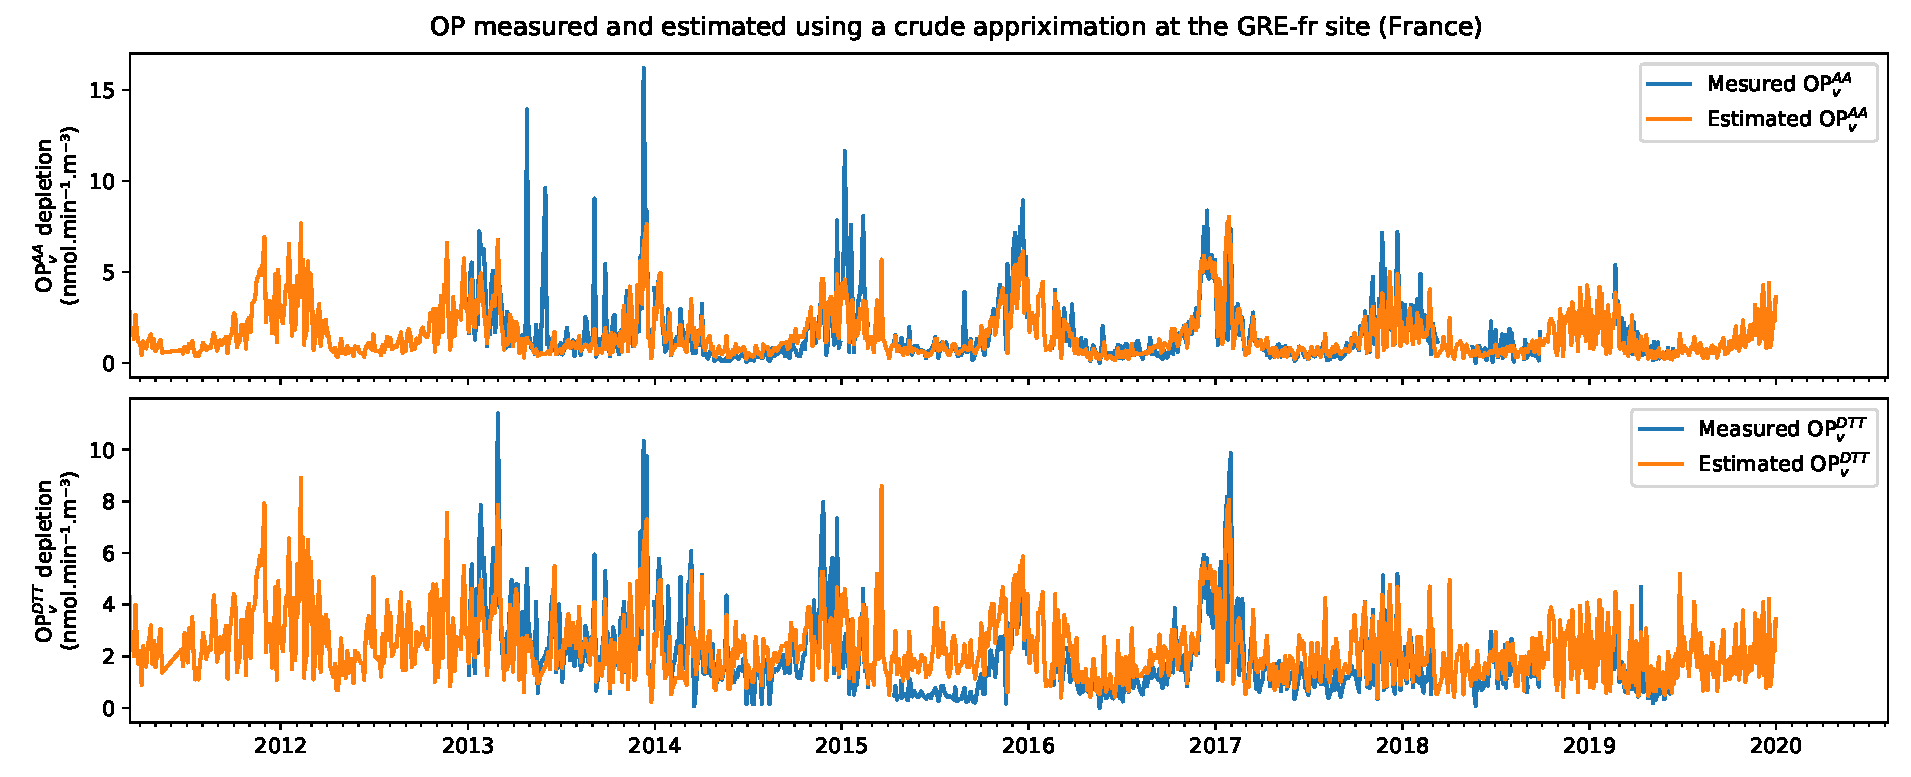
\includegraphics[width=1.0\textwidth]{figures/chapter05/OPGRE-fr_estimated.pdf}
    \caption{\POAAv{} (haut) et \PODTTv{} (bas) estimés en orange et mesurés en bleu sur le site de GRE-fr depuis 2011.}
    \label{fig:OPGRE-fr-estimated}
\end{figure}
 
\begin{figure}[ht]
    \centering
    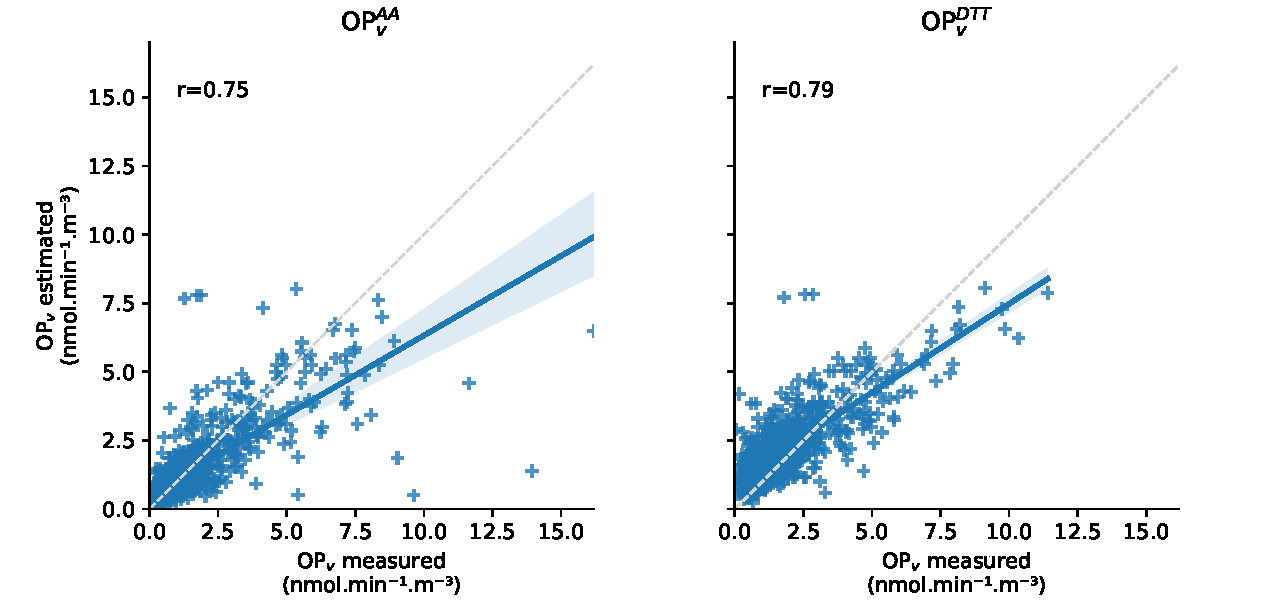
\includegraphics[width=0.8\textwidth]{figures/chapter05/OPGRE-fr_estimated_scatter.pdf}
    \caption{\POAAv{} et \PODTTv{} estimés et mesurés sur le site de GRE-fr depuis 2012.}
    \label{fig:OPGRE-fr-estimated_scatter}
\end{figure}


Il est donc possible d'estimer en premier ordre la contribution des sources majoritaires de
PM aux PO, et ce en prenant en compte l'intégralité des mesure annuelle disponible. La
prise en compte de toutes ces mesures nous affranchi du biais de sélection présent dû
fait de la fréquence d'échantillonage et d'annalyse sur filtre. Les contributions des
sources de PO d'après les mesures journalières d'Atmo AURA sur la station de GRE-fr sont
présentées figure~\ref{fig:OPGRE-fr_source_estimated} et détaillées dans le
tableau~\ref{tab:OPGRE-fr_source_estimated}.

Du fait de l'importance du PO intrinsèque de la source combustion de biomasse
(\textit{Biomass burning} dans le graphique), sa contribution moyenne annuelle est
également importante, notamment pour le \POAAv.  En revanche, puisque l'ont dispose de
l'ensemble des jours de mesures et que cette source présente une dynamique très
saisonnière, l'écart entre contribution moyenne et médiane est très important.
En revanche, conformément aux PO intrinsèque élevés de la source trafic primaire
(\textit{Road traffic} dans le graphique) et sa contribution relativement homogène tout au
long de l'année, cette source est la première contributrice au \PODTTv, aussi bien en
moyenne qu'en médiane.

Si elle n'apprend rien de bien nouveau, cette méthode d'estimation certes grossière,
permet la prise en compte d'un très grand nombre de jours d'observation et met d'autant
mieux en lumière la différence entre contribution moyenne et contribution médiane des
sources de \PMdix{} aux PO.

Enfin, il est possible de propager la variabilité aussi bien de la contribution mensuelle
moyenne de chacune de source que de leur PO intrinsèque dans cette méthode. Ce travail n'a
pas encore été entamé, mais nous disposons de l'ensemble des informations nécessaire pour
cela.

En définitive, puisqu'il est raisonnable d'estimer le PO des \PMdix{} par cette technique,
il parait envisageable d'établir une cartographie du PO à partir soit des mesures satellites
de concentration de \PMdix, soit des sorties de modèle CTM.

\begin{figure}[ht]
    \centering
    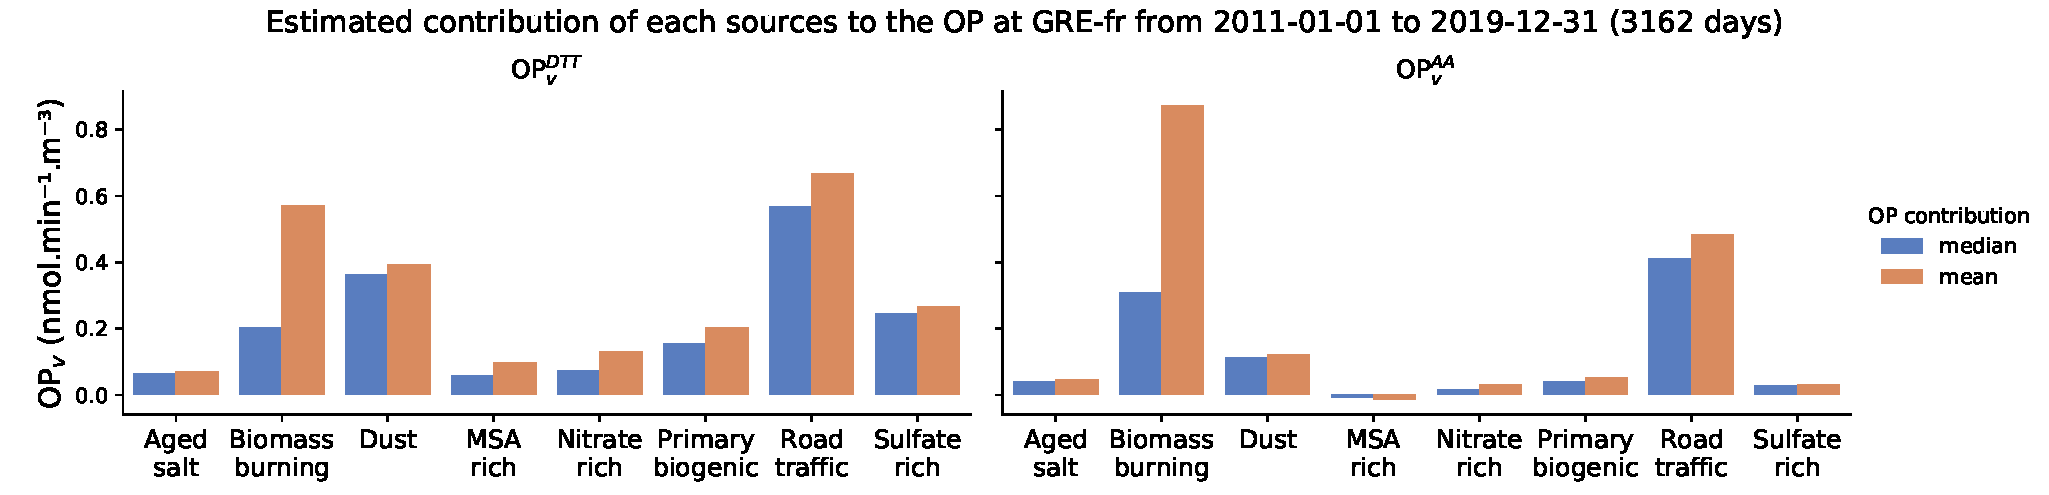
\includegraphics[width=1.0\linewidth]{figures/chapter05/OPGRE-fr_source_estimated.pdf}
    \caption{Contributions estimées moyennes et médianes des sources de \PMdix{} aux
        \PODTTv{} et \POAAv{} sur le site de Grenoble Les frènes entre 2011 et 2019.}%
    \label{fig:OPGRE-fr_source_estimated}
\end{figure}

\begin{table}[ht]
    \centering
    \footnotesize
    \begin{tabular}{cp{1cm}p{1.3cm}p{1.3cm}p{1.3cm}p{1.3cm}p{1.3cm}p{1.3cm}p{1.3cm}p{1.3cm}p{1.3cm}}
        \toprule
        & & \multicolumn{8}{c}{Estimated source contribution to OP in \si{\opv}}\\

                       &      & Aged salt & Biomass burning & Dust  & MSA rich & Nitrate rich & Primary biogenic & Road traffic & Sulfate rich\\\midrule

\multirow{6}{*}{AAv}   & mean & 0.045 & 0.871 & 0.121 & -0.014 & 0.030 & 0.051 & 0.482 & 0.031\\
                       & std  & 0.023 & 1.178 & 0.066 & 0.014  & 0.032 & 0.038 & 0.285 & 0.017\\
                       & min  & 0.002 & 0.008 & 0.005 & -0.114 & 0.001 & 0.001 & 0.041 & 0.001\\
                       & 25\% & 0.028 & 0.066 & 0.074 & -0.020 & 0.007 & 0.021 & 0.275 & 0.019\\
                       & 50\% & 0.041 & 0.308 & 0.111 & -0.008 & 0.016 & 0.038 & 0.409 & 0.028\\
                       & 75\% & 0.058 & 1.265 & 0.158 & -0.004 & 0.042 & 0.072 & 0.626 & 0.041\\
                       & max  & 0.167 & 6.347 & 0.502 & -0.000 & 0.259 & 0.235 & 1.867 & 0.138\\
                          \midrule
 \multirow{6}{*}{DTTv} & mean & 0.070 & 0.571 & 0.392 & 0.096 & 0.131 & 0.202 & 0.668 & 0.266\\
                       & std  & 0.036 & 0.772 & 0.214 & 0.096 & 0.142 & 0.153 & 0.395 & 0.145\\
                       & min  & 0.003 & 0.005 & 0.016 & 0.001 & 0.004 & 0.006 & 0.057 & 0.013\\
                       & 25\% & 0.043 & 0.043 & 0.239 & 0.027 & 0.033 & 0.084 & 0.382 & 0.162\\
                       & 50\% & 0.064 & 0.202 & 0.361 & 0.058 & 0.073 & 0.154 & 0.568 & 0.245\\
                       & 75\% & 0.090 & 0.829 & 0.510 & 0.140 & 0.184 & 0.286 & 0.868 & 0.348\\
                       & max  & 0.261 & 4.162 & 1.623 & 0.772 & 1.129
                       & 0.937 & 2.587 & 1.170\\
                          \bottomrule
    \end{tabular}
    \caption{Contributions estimées des sources de PM aux \POAAv{} et \PODTTv{} pour
    Grenoble Les Frènes entre 2011 et 2019 (n=3162 jours)}
    \label{tab:OPGRE-fr_source_estimated}
\end{table}


\subsection{Prévision déterministe du PO (modélisation CTM)}

Si la partie précédente présentait une méthode approximative de prévision du PO à partir
du calcul de la masse des \PMdix{} estimée par les CTM, il est certainement cependant
préférable d'inclure directement la variable ``potentiel oxydant'' dans ces modèles.

Cependant, le ``PO'' n'étant pas une espèce chimique évoluant et réagissant, son
estimation ne peut se faire que a posteriori et à partir soit du PO intrinsèque de chacune
des espèces chimiques, soit en estimant la contribution des sources à la masse de \PMdix
Mais les mêmes limitations que pour l'inversion par espèces chimiques se retrouve. Il faut donc
réussir à estimer les sources de \PMdix{} dans les modèles CTM.

Ensuite, deux solutions sont envisageables:
\begin{enumerate}
    \item estimer un PO intrinsèque par source d'émission des CTM en utilisant le même
        procédé que celui développée durant cette thèse en utilisant les mesures de PO à
        différentes stations;
    \item établir une équivalence entre source CTM et facteur PMF, puis appliquer les
        PO intrinsèque des facteurs PMF aux sources estimées par CTM.
\end{enumerate}

La première solutions permettrait le prise en compte d'un nombre de source beaucoup plus
grand que celles retenues dans les PMF (émission portuaire, différent type de résidentiel
ou trafic, feu de forêt, etc) puisque les sources des CTM sont fondées sur les SNAP, qui
sont très nombreux.
En revanche, cette solution, dans son implémentation actuelle à travers le ``source
labelling'', ne prend en compte uniquement les sources primaires. Par exemple, la
condensation des NOx du trafic routier et de l'ammoniac de l'agriculture forme du
nitrate-d'ammonium et est attribué selon une moyenne pondérée à la source trafic et
agricole. Il y a donc une perte d'information entre source primaire et secondaire.

La deuxième solution nécessite une comparaison des émissions chimique considérés dans
chacun des SNAP utilisés avec les profils chimiques des facteurs PMF. S'il est possible
d'établir un rapprochement entre ces 2 nomenclatures, il sera possible d'estimer le PO
apporté par ces sources.

Dans les 2 cas, le développement de la technique de ``source-labelling'' et la base de
donnée unique d'attribution des sources en site récepteur appelle à une étude de
sensibilité des prédiction des CTM. Notamment, LOTOS-EUROS\footnote{LOTOS-EUROS:
    \url{https://lotos-euros.tno.nl/}} (abrégé LE) développé au TNO (\textit{Netherlands Organisation for
Applied Scientific Research}) a récemment rendu disponible à travers TOPAS\footnote{TOPAS:
TNO Operational Pollution Apportionment Service (\url{https://topas.tno.nl/})}. Cette
avancée est rendu possible par l'implémentation de \cite{kranenburgSource2013} dans
LOTOS-EUROS v2 \autocite{mandersCurriculum2017}.

Une collaboration entre l'IGE et le TNO a donc été engagée afin de confronter les
prédictions de LE aux sorties PMF. Aussi, dans lors de mon séjour en 2018, nous
avons pu apporté une preuve de concept de la faisabilité de la prédiction du PO par
LE pour 2 sources chimiquement proches entre LE et les PMF.
La figure~\ref{fig:OPmap} présente pour 10 février 2017 à 11:30 la contribution du
transport routier et de la combustion résidentielle à la masse et au \PODTTv{} pour
l'ensemble de l'Europe.

Ce travail, très préliminaire, se poursuivra après ma thèse dans le cadre de cette
collaboration entre l'IGE et le TNO.

\begin{figure}[ht]
    \centering
    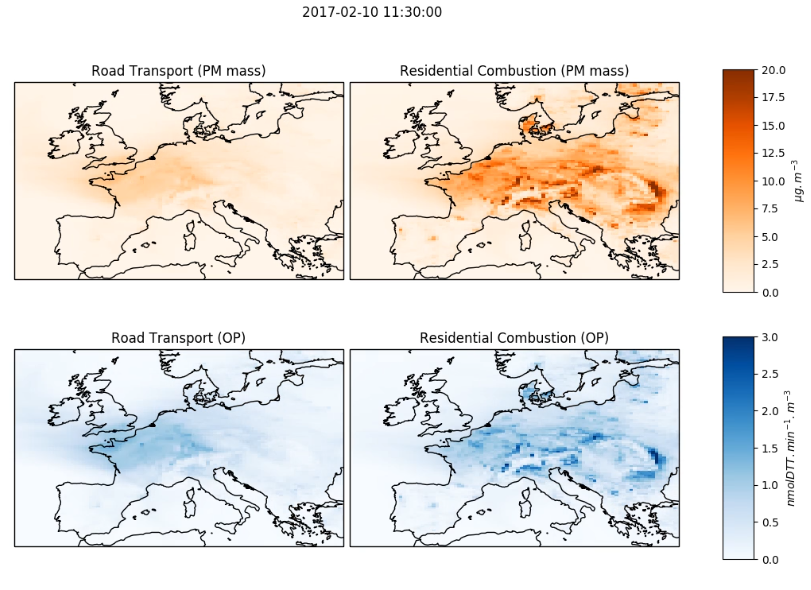
\includegraphics[width=0.8\linewidth]{figures/chapter05/OPmap.png}
    \caption{Preuve de concept de la modélisation grande échelle du potentiel oxydant,
    utilisant le \PODTT{} intrinsèque du trafic routier et de la combustion de biomasse
estimée par \cite{weberSourceinprep.} appliqué aux prévisions de LOTOS-EUROS.}%
    \label{fig:OPmap}
\end{figure}

Cette preuve de concept en 2018 a aiguisé la curiosité des chercheurs et développeurs
d'un autre modèle de chimie transport: Chimère. Chimère a donc maintenant implémenté la
même technique de ``source-labelling'' et un travail identique à celui entamé avec le TNO
et LE est en cours avec le LISA et Chimère. Notamment, de février à juillet 2020, le
stage de M2 de Matthieu Vida portait sur cette thématique, qu'il va poursuivre en thèse à
la rentrée universitaire 2020.

Parallèlement, \cite{daellenbachSourcessubmitted} ont conduit une étude similaire à celle
de \cite{weberSourceinprep.}, mais n'incluant que 109 mesures composites de potentiel
oxydant sur 6 sites de prélèvement en Suisse. Dans cette étude, à laquelle j'ai pris
part, le couplage entre PO intrinsèque et sources déterminée par le CTM CAMx est proposé.
Les résultats obtenus montre une fois de plus
l'importance de la combustion de biomasse mais aussi de la source trafic routière dans
les zones densément peuplées. En estimant l'exposition des populations comme la masse de
\PMdix{} ou la quantité de \POv{} inhalé, cette étude montre une
redistribution complète de l'importance des sources entre concentration massique et
potentiels oxydants. Encore une fois, l'importance du trafic routier s'accroît
considérablement et l'aérosol inorganique, pourtant dominant en terme de masse, n'a plus
qu'une influence minime sur l'exposition aux \POv.

Le même type d'étude, fondée sur une représentativité spatiale et temporelle plus
importante à l'échelle européenne est envisagée dans le cadre de mon
post-doctorat\footnote{sous réserve de validation de cette thèse bien entendu}.

% \begin{figure}[ht]
%     \centering
%     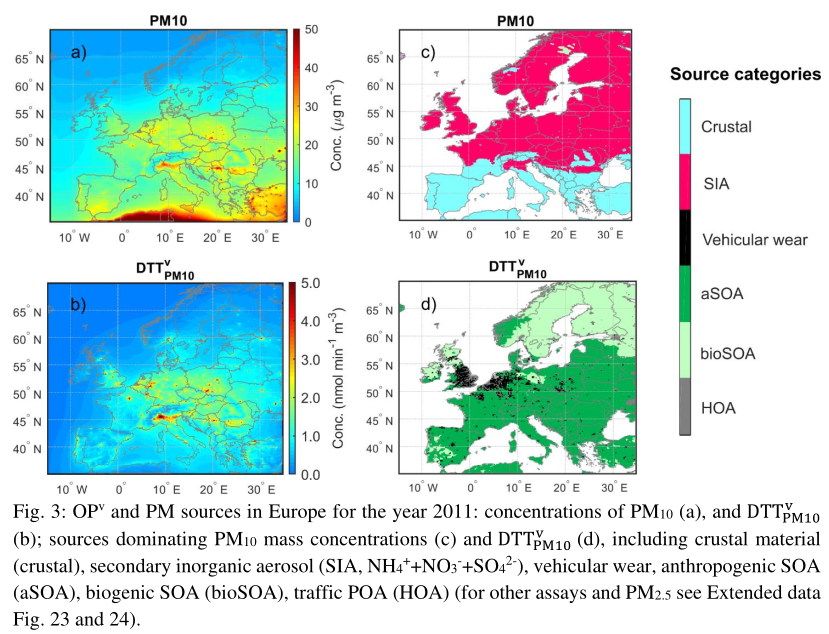
\includegraphics[width=0.8\linewidth]{figures/chapter05/map_kaspard.png}
%     \caption{Estimation européenne du \PODTTv{} et des sources associées par
%     \cite{daellenbachSourcessubmitted}.}%
%     \label{fig:map_kaspard}
% \end{figure}

\section{Contribution non linéarité des sources aux PO : réseaux de neurone}

\subsection{Limitations inhérentes aux modèles linéaires}%
\label{sub:limitations_inhérentes_aux_modèles_linéaires}


Il est connu que la mesure du PO n'est pas linéaire avec la concentrations des composés
chimiques. Il est donc logique de dire qu'il en est de même pour la contribution des
sources.
Or, jusqu'à présent, le PO des sources de PM a été estimé à partir de modèle linéaire,
que ce soit par introduction du \POv{} dans une PMF, par régression linéaire multiple ou
par ACP.
Aussi, aucun terme d'interaction entre sources n'est pris en compte alors même que
le potentiel ``effet cocktail'' entre composés chimiques sur le PO est documenté, comme le
montre la figure~\ref{fig:charrier_hydrogen_2014_fig4} issue de
\cite{charrierHydrogen2014} ou encore 
\cites[figure S7 du supplément]{charrierDithiothreitol2012}{xiongRethinking2017}{samakeUnexpected2017}.

\begin{figure}[ht]
    \centering
    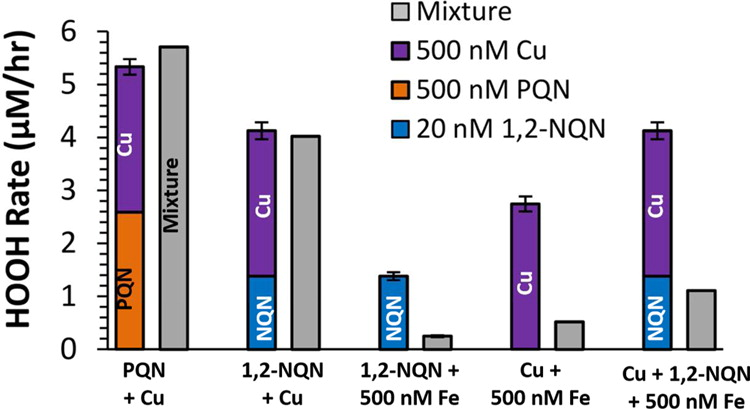
\includegraphics[width=0.5\linewidth]{figures/chapter05/charrier_hydrogen_2014_fig4.jpg}
    \caption{\cite[figure 4]{charrierHydrogen2014}: Initial rates of HOOH production in
    laboratory mixtures of quinones and/or transition metals (gray bars) compared to the
    sum of the rates from the individual redox-active species (stacked colored bars). Error
    bars of the colored stacked bars are the propagated errors of the sum (all have replicate
    samples). The concentrations of metals and quinones are constant: Cu, Fe, and PQN are at
    500 nM, and 1,2-NQN is at 20 nM.}%
    \label{fig:charrier_hydrogen_2014_fig4}
\end{figure}

Si ces modèles permettent une première estimation de la contribution des sources et sont
facilement interprétables, ils présentent donc, par construction, deux biais majeurs: non
prise en compte des effets d'interaction entre sources et non prise en compte de la non
linéarité du PO.

L'ajout de terme d'interaction sous forme de produit des concentrations de sources serait
une solution pour estimer le premier biais, mais le deuxième bien ne peut tout simplement
pas s'estimer par un modèle linéaire. Aussi, l'ajout de terme non linéaires n'est pas
évident car il semble exister une grande diversité de réponses non linéaires selon les
espèces chimiques
considérées~\autocite{charrierDithiothreitol2012,charrierBias2016,calasImportance2017}

Par conséquent, il convient de construire un modèle présentant les caractéristiques
suivantes :
\begin{itemize}
    \item prise en compte de la non-linéarité de la dose-réponse de la concentration des
        sources,
    \item prise en compte d'effets conjoints, potentiellement non linéaire et négatif,
        entres les sources,
    \item ignorant des relations dose-réponse ou entre sources a priori.
\end{itemize}

\subsection{Les réseaux de neurones}%
\label{sub:les_réseaux_de_neurones}

Les réseaux de neurones artificiels (\textit{artificial neural network} ANN) semble être
type de modèle répondant à ces critères. Ils sont plus complexe et flexible que les
modèles linéaire, et sont connu pour être capable de prendre en compte des phénomènes
fortement non linéaires. Aussi, leurs capacités à apprendre des relations complexe et ce
sans aucunes connaissances a priori, simplement en s'entrainant sur un ensemble de données
suffisant, en font un outil très intéressant.
Ce type de modèle a été appliqué avec succès en prévision de la qualité de l'air pour le
\ce{NO2} et les \PMdix{} par~\cite{kukkonenExtensive2003} en comparaison à un modèle
linéaire et déterministe. Dans d'autres disciplinaires des sciences de l'environnement, ce
type de modèle a également montrer son intérêt pour l'évaluation de la qualité de
l'eau~\autocite{nathanApplication2017}.

Formellement, un réseaux de neurones est un graphe orienté pondéré, où lorsque deux
nœuds (ou neurones) sont connectés (i.e lié par un bord orienté du graphe), le résultat en
sortie du neurone devant est utilisé comment entrée du neurone de derrière.
Autrement dit réseau de neurone consiste en une succession de ``nœuds'' (ou synapse, ou
neurone) connectés entres eux pas des relations linéaires appelées ``poids''. Le principe
mimique un réseau de neurone biologique naturelle très simpliste, ou chacune des
informations reçu par un neurone se propage à d'autres neurones, afin de prédire une
valeur finale (par ex. le \POv) en fonction d'un signal initial (par ex. la
concentration massique des sources de PM).
On distingue 3 types de neurones:
\begin{itemize}
    \item neurones d'entrées (input) (connecté aux variables d'entrées),
    \item neurones de sorties (output),
    \item neurones cachés.
\end{itemize}
Le plus couramment utilisés est le \textit{Multi Layer Perceptron} (MLP), qui est un
réseau a-cyclique où les neurones sont structurés en couche successives\footnote{Il est
d'ailleurs montré que le MLP est un approximateur universel}, illustré dans la
figure~\ref{fig:MLP_architecture}.

\begin{figure}[ht]
    \centering
    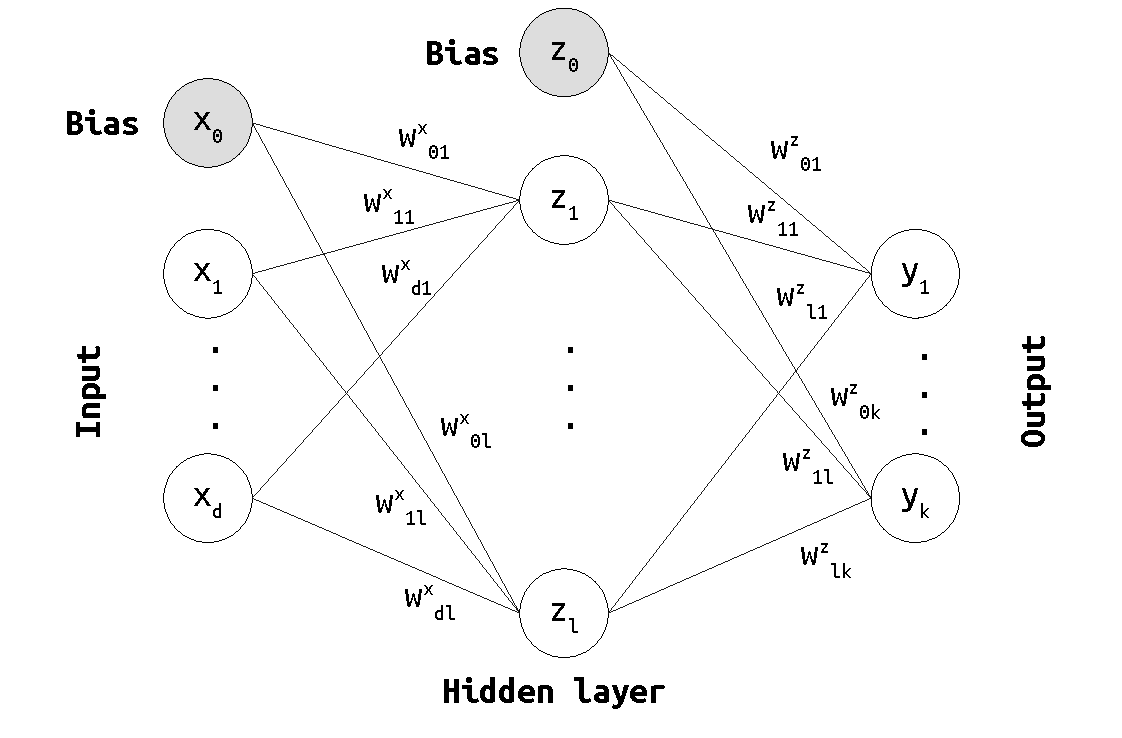
\includegraphics[width=0.7\linewidth]{figures/chapter05/MLP_architecture.pdf}
    \caption{Architecture d'un MLP à une couche cachée, $d$ neurones d'entrée, $l$
    neurones sur la couches cachées et $k$ neurones de sortie (notation d-l-k). $x$
    représente la valeur des variables explicatives (par ex. la concentration massique des
    sources de \PMdix) et $y$ la variable prédite (par ex. le \POAAv{} et \PODTTv).}%
    \label{fig:MLP_architecture}
\end{figure}

Au sein de chaque nœud, l'information reçue est condensée en une valeur unique puis propagée à
son tour aux neurones suivants. En prenant l'exemple du MLP décrit par la
figure~\ref{fig:MLP_architecture}, cette condensation d'information pour la première
couche se fait selon l'Eq.~\ref{eq:ANN_neurone}:
\begin{align}
    \label{eq:ANN_neurone}
    \forall j \in \{1, ..., l\}, z_j &= H\left( \sum_{i=1}^d w^x_{i,j} \times x_i + w^x_{0,j} \right)
\end{align}
avec $w^x_{i,j}$ les poids entre les neurones de la couches d'entrée et cachée, et
$w^x_{0,j}$ représente une constante d'activation pour le neurone $j$. La fonction $H$
peut-être de différents types, mais est très souvent non-linéraire. Le fait de combiner 2
couches de neurone et d'ajouter une fonction d'activation non linéaire amène la
complexité recherché permettant la prise en compte des phénomènes complexes.

Chacun des poids $w$ est inconnu a priori, et sont estimés par processus itératif et
rétro-propagation à partir d'un ensemble de données d'entraînement pour lesquels les
valeurs d'entrées et de sorties sont connues. Les poids sont donc ``appris'' --d'où le
terme de \textit{machine learning}-- par minimisation d'un fonction coût entre prédictions
et observations (de manière similaire à l'algorithme PMF).

En revanche, du fait de leurs complexités, même si les prédictions se trouvent être
correctes, il peut être compliqué d'interpréter le modèle obtenu.


Dans le cadre d'un financement du DataInstitute de l'Université Grenoble Alpes, j'ai
obtenu un financement pour l'encadrement d'un stagiaire de M2, Jean-Baptiste Fiches, afin
de travailler spécifiquement sur ces questions :
\begin{enumerate}
    \item Est-il possible d'appliquer un réseau de neurone pour la prédiction du potentiel
        oxydant ?
    \item Ces réseaux présentent-ils des performances statistiques meilleurs que la
        régression linéaire ?
    \item Est-ce que la non-linéarité attendue est bien observée ?
    \item Comment interpréter ces modèles pour retrouver une information géochimique (i.e.
        PO des différentes sources de PM) ?
\end{enumerate}
Ce travail s'incorporera prochainement dans l'étude de \cite{borlazaUrbaninprep.} du
projet Mobil'Air, afin de comparer les sources de potentiels oxydants sur la
métropole Grenobloise estimer par régression linéaire multiple (MLR) et réseau de neurone
artificiel (MLP).


\subsubsection{Résultats préliminaires}%
\label{ssub:résultats_préliminaires}

Appliqué sur les 3 sites de la métropole Grenobloise, les 2 modèles ont été entraînés sur
\SI{80}{\percent} des données et testés sur les \SI{20}{\percent} restant. Les performances
statistiques des deux types de modèles (MLP et MLR) sont relativement
similaires (figure~\ref{fig:perfMLPMLR}) et chacun des deux modèles prédit chaque \POv{}
(mesuré par AA, DTT et DCFH) sur les 3 sites avec relativement les mêmes performances.
Ce type de modèle permet donc d'expliquer au moins aussi bien que le MLR les PO à partir
des sources d'émissions de \PMdix.

\begin{figure}[ht]
    \centering
    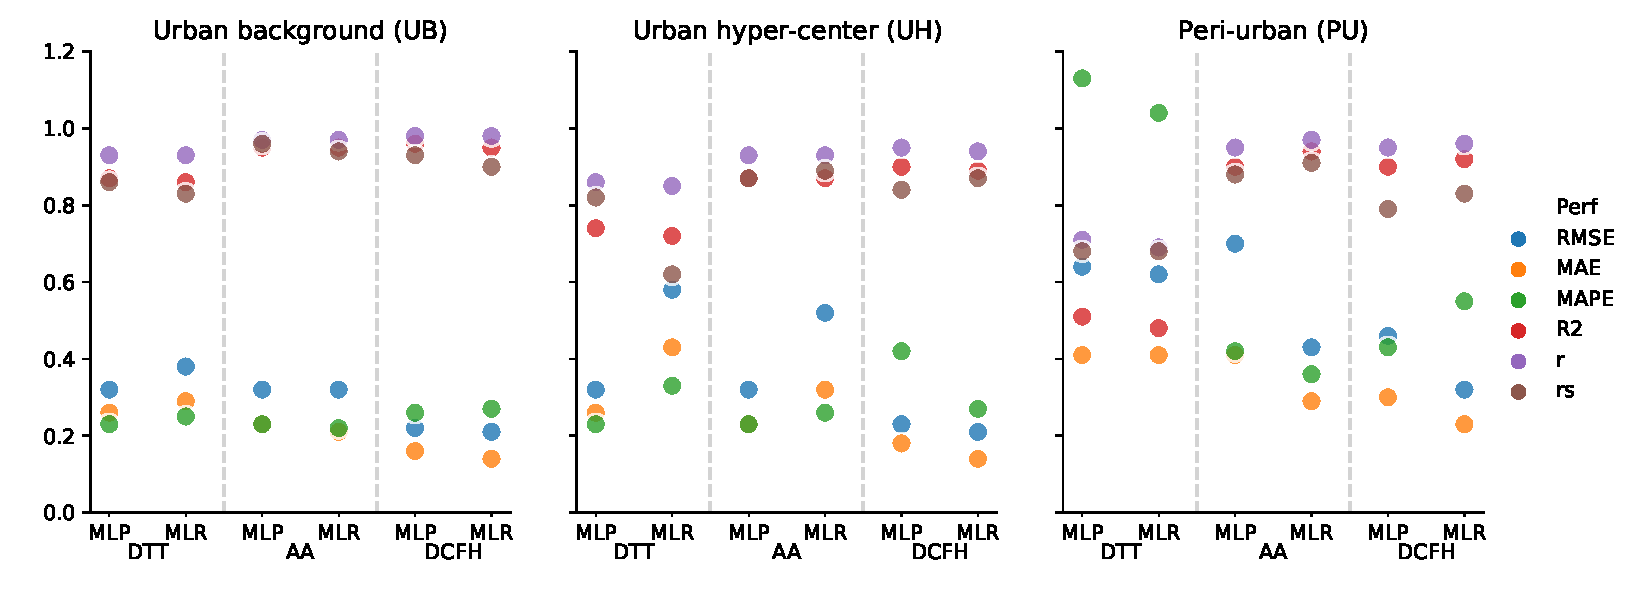
\includegraphics[width=1.0\linewidth]{figures/chapter05/perfMLPMLR.pdf}
    \caption{Performances statistiques des prédictions du modèle MLR et MLP sur les 3
    sites de Grenoble \autocite{borlazaUrbaninprep.}. (UB = GRE-fr, UH = GRE-cb, PU = Vif)}%
    \label{fig:perfMLPMLR}
\end{figure}

Pour estimer si le MLP capture bien des relations non-linéaire, 2 expériences sont menées.
Dans les deux cas, le MLP est entraîne sur le jeu de données du site de GRE-fr. Deux
situations fictives sont ensuite imaginées.

La première consiste à estimer le \PODTTv{} par le MLP, toutes contributions des sources
nulles sauf une, variant de 0 à 24~\si{\ugm}. La réponse du \PODTTv{} en fonction de
l'augmentation linéaire de la contribution de chacune des sources est présentée
figure~\ref{fig:figures/chapter05/10sourcesLinearite}. On y observe bien une réponse
non-linéaire en fonction d'une augmentation linéaire de la contributions de
chaque source. On note par ailleurs dans ce modèle un biais constant de l'ordre de
\SI{-0.5}{\opv} lorsqu'aucune source n'est présente.
On remarque également l'influence négative des sources primaire biogénique, nitrate-rich
et MSA-rich (i.e Marine SOA dans la figure) mais aussi la forte influence de la source
trafic primaire et industrielle.
\todo{je n'arrive pas à tout distinguer sur cette figure. J'ai demandé à JB de la refaire.
En attente}

Dans la deuxième situation, on cherche à estimer si le MLP prévoit des effets non-additif
lors de la présence conjointe de plusieurs sources de \PMdix. L'expérience prédit donc le
\PODTTv{} pour un ensemble d'échantillons de test où cette fois 2 sources présentes des
concentration variant chacune de 0 à \SI{10}{\ugm}. Les résultats sont encore attendus,
mais si l'effet est additif, le gradient de l'augmentation du \PODTTv{} dans un espace en
2 dimensions représentant la contribution de chacune des sources est sensé être linéaire.
Dans le cas contraire, cela indiquera un effet cocktail entre ces 2 sources.

\begin{figure}[ht]
    \centering
    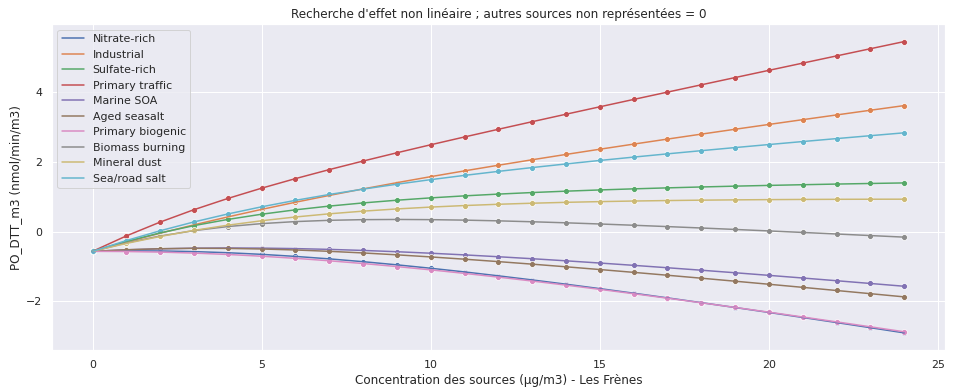
\includegraphics[width=0.8\linewidth]{figures/chapter05/10sourcesLinearite.PNG}
    \caption{Effet non linéaire de l'augmentation de la concentration d'une source
        d'émission sur le \PODTTv{} d'après un réseau de neurone entraîné sur GRE-fr. Source: \cite{fichesMachine2020}.}%
    \label{fig:figures/chapter05/10sourcesLinearite}
\end{figure}

Enfin, il se pose la question de l'estimation de la contribution des sources aux PO. Du
fait de la complexité du modèle, il n'est pas possible d'attribuer \emph{un} PO
intrinsèque par source, celui-ci étant changeant en fonction d'autres paramètres.
La technique utilisée est donc similaire à celle présentée
en~\ref{par:source_apportionment} dite de \textit{brute-force} pour les CTM. À une
simulation de référence pour laquelle toutes les sources sont prisent en compte est
soustrait différentes simulations où une sources est mise artificiellement à une
contribution nulle.  La différence nous apprend donc quel aurait été le \POv{} en
l'absence de chacune des sources.
Cette technique permet donc de répondre à la question
\begin{quote}
   Si les émissions de cette source sont diminuées ou supprimées, quels impacts cela va-t-il
   avoir sur le \POv{} final ?
\end{quote}
mais ne répond en revanche pas à
\begin{quote}
   Dans la concentration ambiante de PM, à combien s'estime la contribution de cette source
   d'émission ?
\end{quote}

De même, cette étude est actuellement en cours au sein du stage de Jean-Baptiste Fiches
que j'encadre et de \cite{borlazaUrbaninprep.}.

\section{Exposition et épidémiologie}

La mesure du PO et son application outil de mesure de la qualité de l'air demande
nécessairement des études sur la capacités prédictives des PO sur les impacts sanitaires.
Aussi, dans le mode de vie occidental, nous passons le plus clair de notre temps en espace
clos intérieur (maison ou travail
principalement)~\autocite{netheryTime2009,ouidirEstimation2015}. La qualité de l'air
mesuré dans les stations conventionnelles n'est donc peut-être pas représentative de
l'exposition réelle des individus~\autocite{sauvainOxidative2015}.

\subsection{Mesures intérieure et personnelle}

Sur Grenoble, après une étude pilote de \cite{ouidirEstimation2015} portant sur
l'exposition personnelle de 40 femmes enceintes, le projet
SEPAGES~\autocite{lyon-caenDeciphering2019} a pour ambition la mesure d'un très large
ensemble de marqueurs phénotypiques pour un corpus d'environ 480 couple mères-enfants
suivis pendant leur grossesses et des premières années des enfants. Parallèlement,
l'exposôme est mesuré très finement, prenant en compte l'exposition personnelle des
sujets dès le premier trimestre de la grossesse grâce au port de micro-capteurs autonomes.

Grâce au projet Mobil'air, en plus des \ce{NO2} et masse des \PMdc, le PO a également été
mesurés sur ces micro-filtres\footnote{Les faibles masses prélevées ont fait l'objet
    d'une adaptation méthodologique sur la mesure du PO afin de réduire les seuils de
quantification de ces tests.}.
Aussi, des échantillons d'air intérieur pour 140 foyers pour deux périodes entre 2018 et
2019 ont été prélevés dans l'agglomération grenobloise. Cela représente un total de 280
échantillons de fraction \PMdc{} pour sur lesquels une chimie détaillée et les PO sont en
cours d'analyse. Une partie déjà analysées des mesures de carbone organique est présentée
figure~\ref{fig:figures/chapter05/OC_mobilair}, confrontée au mesure extérieur sur la
station de GRE-fr d'Atmo AURA pour la même période. De même que pour les mesures extérieures,
une saisonnalité des mesures intérieure est retrouvée.
En revanche, il existe
des échantillons où la concentration intérieure est plus élevées que celle extérieure,
alors même que seule la fraction \PMdc{} est prise en compte pour les mesures intérieures.

\begin{figure}[ht]
    \centering
    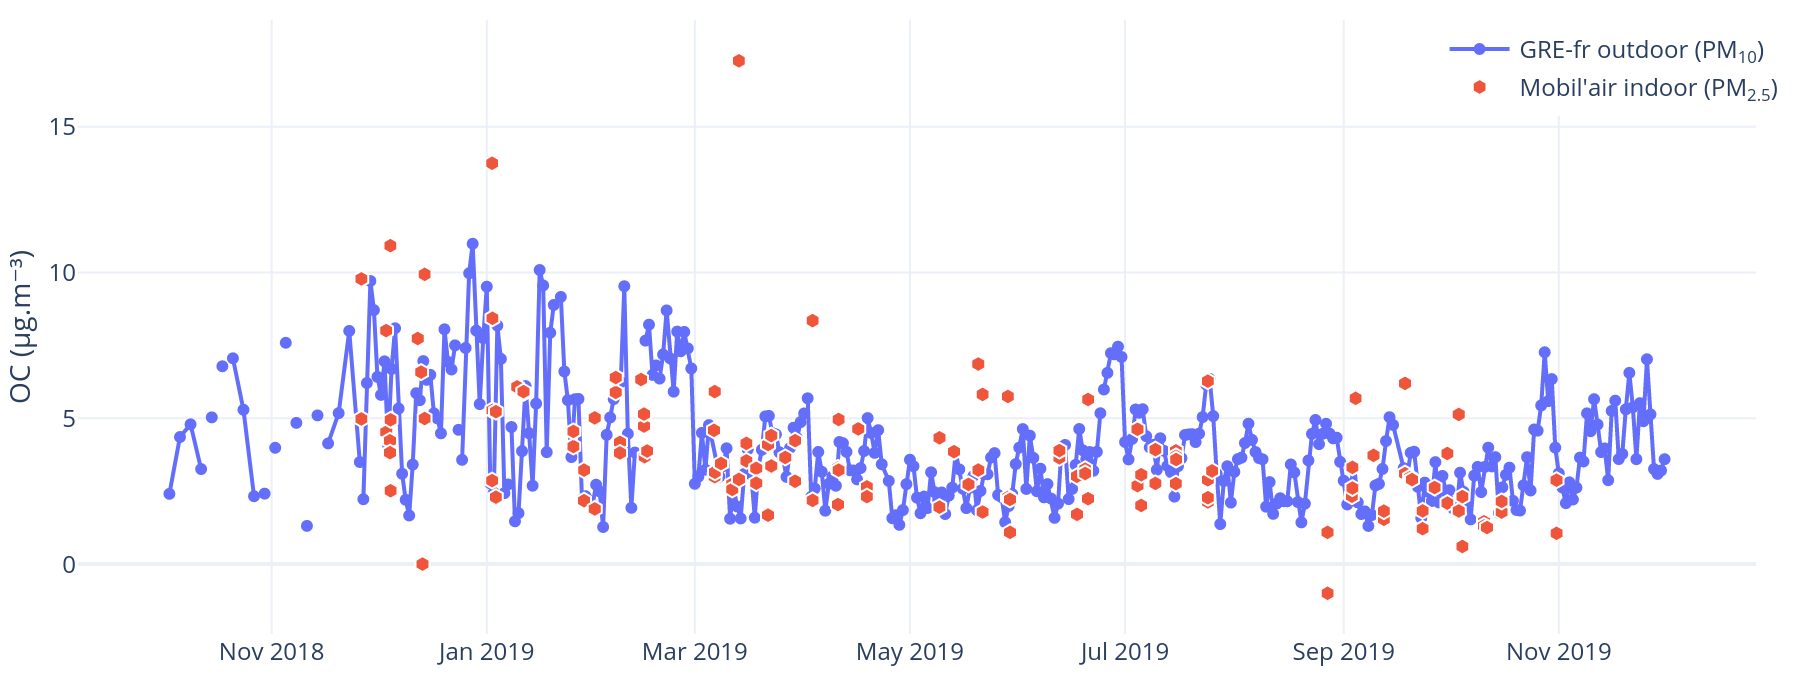
\includegraphics[width=1.\linewidth]{figures/chapter05/OC_mobilair.png}
    \caption{Mesure de l'OC en air extérieur (station de GRE-fr) et intérieur chez les
    participants de l'étude sur la métropole grenobloise.}%
    \label{fig:figures/chapter05/OC_mobilair}
\end{figure}

Concernant les mesures personnelles, la figure~\ref{fig:figures/chapter05/personnal_OP}
présentes la confrontation des mesures de la station GRE-fr et personnelles pour l'année
2015, 2016 et 2017. Bien que l'on observe toujours un cycle saisonnier pour le \POAAv{} et
\PODTTv{} personnel, son amplitude est plus faible que celui du \POv{} d'extérieur. Aussi,
alors que l'on a montrée dans section~\ref{sub:pm10_pm2_5} que le \POv{} des \PMdc{} est
toujours plus faible que celui des \PMdix{} lorsqu'il proviennent de la même station de
prélèvement, ce résultat n'est pas retrouvé pour le \POv{} personnel. Notamment, le \POv{}
personnel en été est plus élevés que le \POv{} de l'air extérieur, indiquant des sources
de PO différente entre air extérieur et air ``personnel''.

\begin{figure}[ht]
    \centering
    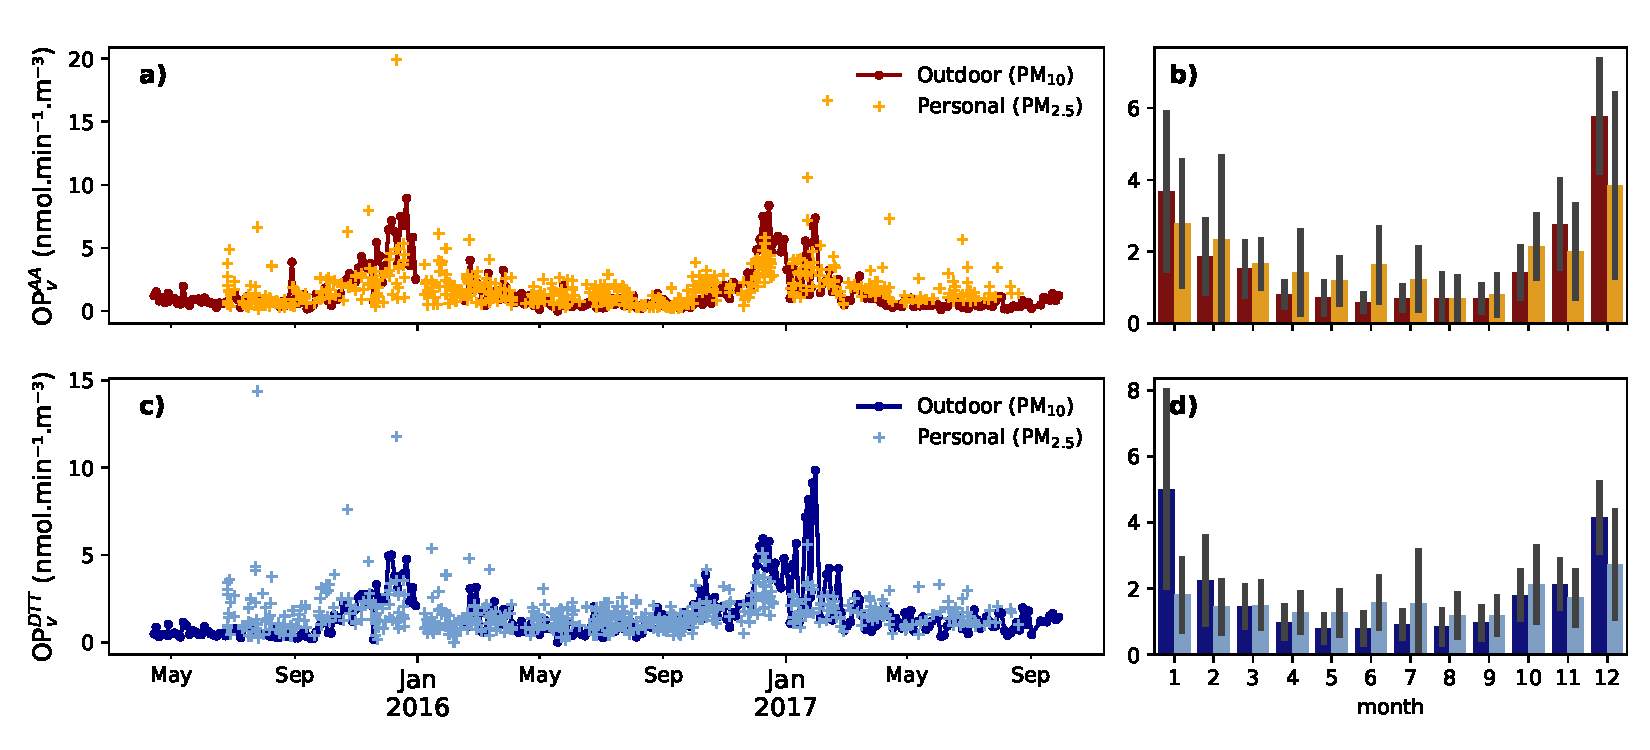
\includegraphics[width=1.0\linewidth]{figures/chapter05/personnal_OP.pdf}
    \caption{Mesures de \POAAv{} et \PODTTv{} en extérieur (station GRE-fr) et
    personnelles des sujets de la cohortes SEPAGES. La moyenne et l'écart type par mois
sont présentés en b) pour le \POAAv{} et d) pour le \PODTTv. L'orange représente le
\POAAv{} et le bleu le \PODTTv{}. Les prélèvements en extérieur sont en foncés et personel
en clairs.}%
    \label{fig:figures/chapter05/personnal_OP}
\end{figure}

\subsection{Étude épidémiologique -- cohorte SEPAGES}

La cohortes SEPAGES nous permet une caractérisation précise de l'exposition personnelle
maternelle en lien avec un ensemble conséquent de variables phénotypiques du nouveau-né.
De façons similaire à l'étude de \cite{ouidirEstimation2015}, l'effet de l'exposition aux
\ce{NO2}, concentration massique des \PMdc mais surtout aux \POAAv{} et \PODTTv{} est en
cours d'étude par \cite{borlazaPersonalinprep.}.
Grâce à cette étude, le pouvoir prédictif de la métrique de la masse ou du PO des \PMdc{}
sur le petit poids de naissance ou la circonférence crânienne, parmi d'autres variables,
pourra être évaluer.

De même, la thèse d'Anouk Marshal débutant à l'automne 2020 aura pour objectif d'établir
un modèle de \textit{land use regression} (LUR) sur Grenoble et périphérie afin de
quantifier l'importance de l'environnement géographique pour la mesure du PO et
l'exposition personnel, en lien avec les effets sanitaires observées dans la
cohortes SEPAGES.


